\documentclass[pra,twocolumn,preprintnumbers,amsmath,amssymb,nofootinbib,floatfix,longbibliography]{revtex4}

\usepackage{graphicx, bm, tikz, braket, mathrsfs, comment}
\usepackage[breaklinks]{hyperref}
\usepackage{gensymb} %\degree

\makeatletter

\def\graphicscale{\twocolumn@sw{0.3}{0.4}}
\def\graphicthreescale{\twocolumn@sw{0.3}{0.4}}
\newcommand{\rev}[1]{\textcolor{red}{#1}}

\begin{document}

\title{Notes}

\author{}
\affiliation{}

%\date{}

\begin{abstract}
\end{abstract}
\maketitle

\section{Model}

As a paradigmatic model, we consider a fermionic lattice
system described by the Kitaev Hamiltonian with Open
Boundary Condition(OBC)~\cite{K01}:

\begin{equation}
	\label{HKitaev}
	\hat H(\mu)=-\mu_i \sum_{x=1}^L\hat c_x^\dagger\hat c_x
    -\sum_{x=1}^{L-1} \Bigr[\hat c_x^\dagger \hat c_{x+1} +
	\hat c_x \hat c_{x+1} + {\rm h.c.} \Bigr]  \,\,;
\end{equation}

where the operator $\hat c_x^\dagger$ $(\hat c_x)$ creates
(annihilates) a spinless fermion in the $x$-site of the
wire. This operators satisfy the anticommutation relations,
i.e. $\{\hat c_x^\dagger, \hat c_y\} = \delta_{x,y}$ and
$\{\hat c_x, \hat c_y\} = 0$. Moreover, the parameter $\mu$
represents the chemical potential of the system.\\
This model is exactly mapped in the quantum Ising model by
a Jordan-Wigner transformation in which we associated the
parameter $\mu$ with the transverse field.\\
Like in the Ising chain, the lattice Kitaev model undergoes
a Continuous Quantum Transition (CQT), at the critical
point $\mu_c = -2$, belonging at the universality class of
the two-dimensional classical Ising model. Indeed, the
correlation length, close to the critical point, diverges
as $\xi \sim |\mu - \mu_c|^{-\nu}$, with the critical
exponent $\nu$ equal to $\nu = 1$. While the lowest energy
gap $\Delta$ vanishes as $\xi ^{-z}$, where $z=1$ is the
dynamical critical exponent.\\
We analyze the effect of two different mechanisms which
control the out-of-equilibrium dynamics:

\subparagraph{Unitary Quench Mechanism}$ $\\
  Where the time evolution of the system density matrix
  $\rho$ is given by:
  \begin{equation}
    \label{unitrhot}
    \frac{d \rho}{d t} = -i
    \bigr[ \hat H, \rho \bigr] \,\,.
  \end{equation}
  The Hamiltonian $H$ starts from the Kitaev Hamiltonian
  (\ref{HKitaev}) with $\mu = \mu_i$, then we change
  suddenly the value of the chemical potential $\mu_i$
  to a final value $\mu_f$.

\subparagraph{Dissipative Mechanism}$ $\\
  In this case, each system site is coupled with uniform
  and identical thermal baths with temperature $T_b$; using
  the Born-Markov and secular approximation, the time
  derivative of the density matrix $\rho$ obeys to the
  Lindblad master equation~\cite{BP07}:
  \begin{equation}
    \label{Lindblad}
    \frac{d\rho}{dt} = \mathcal{L}[\rho]\equiv
    -i\bigr[\hat{H},{\rho}\bigr]+\mathbb{D}_{T_b}[\rho]\,,
  \end{equation}
  where $\mathcal{L}$ is the Liouvillian superoperator, and
  $\mathbb{D}$ is the corresponding dissipation term, whose
  strength is regulated by the homogeneous coupling
  $\gamma$:
  \begin{align}
    \label{dissipator}
    \mathbb{D}_{T_b}[\rho]&=
    \gamma \sum_{x=1}^{L}\mathbb{D}_{x}[\rho]\,.
  \end{align}
  The form of the dissipator $\mathbb{D}$ is associated
  with the Bogoliubov base which diagonalizes the
  Hamiltonian reported in the Eq. (\ref{HKitaev}). This
  type of interaction is chosen by introducing an
  interaction Hamiltonian term between the baths and the
  fermionic system particles. Using the Born-Markov
  approximation, we can estimate the dissipation evolution
  in therms of the Lindblad formalism. \\
  The equilibrium steady state (ESS) solution, obtained in
  the limit $t \to +\infty$, is achieved after this
  thermalization process. This state must correspond to the
  Gibbs state associated with the temperature
  $T_i=\beta_i^{-1}$.\\
  From this condition, we can compute the ESS correlation
  values starting from the diagonalized form of the
  Hamiltonian \ref{HKitaev}:
  \begin{equation}
    \label{HKdiag}
    H(\mu)=\sum _{j=1}^L\,\omega _j \,\hat b^\dagger _j\,
    \hat b_j+ \frac{1}{2}\,\Bigr[ -2L\mu - \sum _{r=1}^L
    \omega _r \Bigr] \,\,;
  \end{equation}
  where the $\omega_k$ is the spectrum of the Bogoliubov
  fermion eigenoperators $\hat b_k$.\\
  We can assume the quasi-particles associated with $b_k$
  as a free fermion gas in which the partition function is:
  \begin{equation}
    \label{Partition}
    {\cal Z} = {\rm Tr} \,\, e^{-\beta_i
      \sum_j \omega _j \,\hat b^\dagger _j\, \hat b_j}\,\,;
  \end{equation}
  less than constant terms.\\
  Since Eq. (\ref{Lindblad}) represents a thermalization
  process, its large-time limit must correspond with the
  Gibbs state at the temperature $T_i$. In this state, the
  correlation functions $\braket{b^\dagger_k b_k}$
  can be derived by the following relation:
  \begin{align}
    \label{Zcorr}
    \braket{b^\dagger_k b_k} =
    {\rm Tr} \Biggr[ \frac{b^\dagger_k b_k}
                    {\cal Z}e^{-\beta_i \hat H} \Biggr]
    = -\frac{1}{\beta_i}\partial_{\omega_k}\ln{\cal Z}\,\,;
  \end{align}
  where we use that the Gibbs state is equal to
  $\hat \rho = e^{-\beta_i\hat H(\mu)}/{\cal Z}$. To
  compute the ${\cal Z}$ function, we consider all the
  basis vector in the Hilbert space associated with the
  free quasi-particle fermions. In this way:
  \begin{equation}
    {\cal Z} = \prod _{j=1}^L
    \Bigl( 1 + e^{-\beta_i \omega_j} \Bigl) \,\,;
  \end{equation}
  and from Eq. (\ref{Zcorr}):
  \begin{align}
    \braket{b^\dagger_k b_k}= &
    -\frac{1}{\beta_i}\partial_{\omega_k} \sum _{j=1}^L
    \ln\Bigl( 1 + e^{-\beta_i \omega_j} \Bigl)= \\
    = &  \frac{e^{-\beta_i \omega_k}}
            { 1 + e^{-\beta_i \omega_k} } =
    \frac{1}{1 + e^{\beta_i \omega_k}}
    \,\,;
  \end{align}
  where $f(\omega_k) = 1 / (1 + e^{\beta_i \omega_k})$ is
  the statistical Fermi-Dirac distribution function. The
  non-diagonal term

\section{Observables}
\label{observables}

To monitor the out-of-equilibrium dynamics, close to the
critical point, we introduce the two-point correlations
functions as:
\begin{align}
  \label{Ccorrs}
  C(x,y) &={\rm Tr}\Bigr[\rho \hat c^\dagger_x \hat c_y
						+  {\rm h.c.}\Bigr]\,\,,\\
  \label{Pcorrs}
  P(x,y) &={\rm Tr}\Bigr[\rho \hat c_x\hat c_y +
    {\rm h.c.}\Bigr] \,\,;
\end{align}
these observables are local and depend from the site
position in which we compute the correlations. They are an
optimal choice to investigate the early-time regime and the
stationary behavior of the lattice system. \\
To simplify the notation, we define the following auxiliary
variables $\mathscr{C}$ and $\mathscr{P}$ defined as:
\begin{align}
  \label{RedCorr}
  \mathscr{C}_{x,y} &= {\rm Tr}\Bigr[\rho \hat c^\dagger_x
    \hat c_y\Bigr]\,\,,\\
  \mathscr{P}_{x,y} &= {\rm Tr}\Bigr[\rho \hat c^\dagger_x
    \hat c^\dagger_y\Bigr]\,\,.
\end{align}
In some case, it is useful to analyze quantities which are
independent by the site of the wire. In particular, the
particle density $D$ is a global observable defined as:
\begin{equation}
  \label{partdens}
  \hat D = \frac{1}{L}
  \sum _x \hat c_x^\dagger \hat c_x \,\,.
\end{equation}
To study its time-evolution, we consider the difference $N$
between the value of $\hat D$ at the time $t$ and its value
at the critical point $\mu_c,\,\,T=0$. In other words, if
we define the density matrix $\rho(t)$ at the time $t$ and
$\rho_c$ at the point $\mu = \mu_c$ with temperature $T=0$,
$N$ is equal to:
\begin{equation}
  \label{Nobs}
  N(t) = {\rm Tr}[\rho(t)\hat D]- {\rm Tr}[\rho_c \hat D]
  =\frac{{\rm Tr}[\rho(t)\hat c_x^\dagger \hat c_x] -
      {\rm Tr}[\rho_c \hat c_x^\dagger \hat c_x]}{L} \,\,;
\end{equation}
where $\rho_c$ is the density matrix at the critical point
$\mu=\mu_c$.

\section{Protocol}

Now, let us specify how we prepare the initial quantum
state and how we define the time evolution protocol:
\begin{itemize}
  \item
  At first, we keep the chemical potential $\mu_i$ fixed,
  then we take as initial state the Gibbs state:
  \begin{align}
	\label{Gibbs}
	\hat \rho_i  = \frac{1}{\cal Z} \,\,&
	e^{-\beta_i \hat H_K(\mu_i)} \,\,,\\
    {\cal Z} = {\rm Tr} \,\,e^{-\beta_i } \,\,, & \qquad
	\beta_i  = \frac{1}{T_i} \,\,;
  \end{align}
  where we chose the parameter $\mu_i$ close to the
  critical point $\mu_c$.

  \item
  Then, we consider two different cases:
  \begin{itemize}
    \item[(i)]
    in one, we realize a unitary quench protocol with a
    sudden change of the chemical potential to a value
    $\mu_f$;

    \item[(ii)]
    in the latter, we switch on, also, the dissipation
    coupling constant which tunes the interaction strength
    with a set of homogeneous thermal with temperature
    $T_b$; the time-evolution of the density matrix derives
    from the Eq. (\ref{Lindblad}).
  \end{itemize}

  \item
  In each time step, we evaluate the observables reported
  in the section \ref{observables} to analyze their
  out-of-equilibrium behavior.
\end{itemize}



\section{Initial Gibbs State}

Since we take the Kitaev chain in
equilibrium with the temperature $T_i$, the initial density
matrix corresponds with the Gibbs mixture in the Eq.
(\ref{Gibbs}).\\
In this way, however, we must use all the Hilbert space to
build our density matrix $\rho_i$ obtaining results only
for small values of the system size.\\
We can simplify the problem if we compute directly the
correlation matrix associated with the correlation function
in Eqs. (\ref{Ccorrs}) and (\ref{Pcorrs}). In the following
we put the details of the derivation.\\
\medskip
The Hamiltonian (\ref{HKitaev}) is quadratic in the operators $\hat c,\,\hat c^\dagger$ and it can be diagonalized with a Bogoliubov transformation~\cite{BGN88}:
\begin{equation}
  \label{Hdiag}
  H(\mu_i)=\sum _{k=1}^L\,\omega _k \,\hat b^\dagger _k\,
  \hat b_k+ \frac{1}{2}\,\Bigr[ -2L\mu_i - \sum _{r=1}^L
  \omega _r \Bigr] \,\,;
\end{equation}
where the $\omega_k$ is the spectrum of the Bogoliubov
eigenoperators $\hat b_k$.\\
The correlation function associated with the Bogoliubov
operators, evaluated in the Gibbs state, are obtained by
doing the limit $t \to +\infty$ on the solution of the
following master equation~\cite{PCD22, DR21}:
\begin{align}
   \label{EQLindblad}
   \frac{d O_{H}(t) }{d t}  &= i\,\Bigr[\hat H,
      O_{H}(t) \Bigr] + \mathbb{D}[O_{H}(t)]\,\,,\\
  \mathbb{D}[O_H(t)] =
  \,\,\gamma \sum _k &
  f(\omega_k)\,\biggr[2\hat b_{k}^\dagger O_H(t)\hat b_{k}-
  \Bigl\{ O_H(t), \, \hat b_{k} \hat b_{k}^\dagger \Bigl\}
  \biggr]  + \notag\\
  +\gamma \sum_k  (1-f(\omega_k)) &
  \,\biggr[ 2\hat b_{k} O_H(t) \hat b_{k}^\dagger - \Bigl\{
  O_H(t), \, \hat b_{k}^\dagger \hat b_{k} \Bigl\} \biggr]
\end{align}
in which we have:
\begin{align}
  f(\omega_k) &= (1 + e^{\omega_k/T_i})^{-1} \,\,;\\
  O_H(t) &= \Bigl(b^\dagger_k b_q\Bigl)_H\,\,.
\end{align}
The correlation operator $O_{H}(t)$ is written in
Heisenberg picture and we can write similar equations for
$b_k b^\dagger_q$, $b^\dagger_k b^\dagger_q$, $b_k b_q$. \\
The mean value of this operators in the Gibbs state is
given by doing the trace of the operator in Eq.
(\ref{EQLindblad}) and taking $t\to +\infty$ in its
solution. The only contribution different by zero is:
\begin{equation}
  \label{BogCorrInit}
  \braket{b^\dagger_k b_q} = \delta_{k,q} f(\omega_k) \,\,.
\end{equation}
In this change of basis, the
Bogoliubov operators $\hat b$ are represented by a linear
combination of $\hat c,\,\hat c^\dagger$ whose coefficients
are strictly associated with the correlation matrix of the
system.
To evaluate the correlations (\ref{Ccorrs})-(\ref{Pcorrs}),
we write:
\begin{equation}
  \label{transBogol}
  \hat c_x = \sum_{k=1}^L A_{xk} b_k + B_{xk} b^\dagger_k
  \,\,;
\end{equation}
therefore:
\begin{align}
  \label{initcorr}
   C(x,y) = \sum_{k,q=1}^L
  A^*_{xk}A_{yq} \braket{b^\dagger_k b_q}
  + B^*_{xk} B_{yq} \braket{b_k b^\dagger_q} + \notag\\
  A^*_{xk} B_{yq} \braket{b^\dagger_k b^\dagger_q} +
  B^*_{xk} A_{yq} \braket{b_k b_q}
  \,\,;
\end{align}
\medskip


\section{Out-of-equilibrium dynamics}

\subsection{Unitary dynamics}

\begin{figure}[!htb]
  \includegraphics[width=0.95\columnwidth]
  {figs/LCk-1q0e100g0.pdf}
  \includegraphics[width=0.95\columnwidth]
  {figs/LPk-1q0e100g0.pdf}
  \includegraphics[width=0.95\columnwidth]
  {figs/LNk-1q0e100g0.pdf}
  \caption{Scaling behavior of the two-points
    correlations functions $C(x,y,t)$ (top), $P(x,y,t)$
    (center) and the subtracted particle density $N(t)$
    (bottom) for $x=L/3$, $y=2L/3$  keeping the scaling
    variables $\kappa_i=-1$, $\kappa=0$, $\Xi = 1$ fixed in
    function of $\Theta = tL^{-z}$, up to system size
    $L=120$.}
  \label{qthk0q2e1}
\end{figure}

Starting from the Gibbs state introduced above, at $t=0$,
 we perform a quench protocol on the Hamiltonian
(\ref{HKitaev}) from an
initial value to another one. This process lead to a
reformulation of the Bogoliubov bases in which the time
evolution operator acts. \\
This operator is unitary because the state is not in
contact with any thermal bath. The correlation functions
are achieved from the solution:
\begin{align}
   \label{EQUnitary}
   \frac{d O_{H}(t) }{d t}  &= i\,\Bigr[\hat H,
      O_{H}(t) \Bigr] ;\\
    O_H &= \Bigl(c^\dagger_x c_y\Bigl)_H\,\,.
\end{align}
where the initial condition are given by Eq.
(\ref{initcorr}).\\
Indeed, using the anti-commutation relations and the
Hamiltonian $\hat H(\mu_f)$, the time-evolution of the
2-point correlation functions $C$ and $P$ can be expressed
as:
\begin{align}
C(x,y,t) & =  2\,{\rm Re}\Bigr[
\,{\mathscr{C}_{x,y}}(t) \,\Bigr]        \,\,, \\
P(x,y,t) & = 2\,{\rm Re}\Bigr[
\,{\mathscr{P}_{x,y}}(t) \Bigr]   \,\,.
\end{align}
where this functions evolves in the following
way~\cite{TV21}:
\begin{align}
\frac{d\mathscr{C}_{x,y}}{dt}& =
i\,\bigr[\mathscr{C}_{x,y+1} - \mathscr{C}_{x-1,y} +
\mathscr{C}_{x,y-1} - \mathscr{C}_{x+1,y} \bigr] - \notag\\
-i\, \Bigl(& \mathscr{P}_{y,x-1}^\dagger -
\mathscr{P}_{y,x+1}^\dagger \Bigl)  + i\, \Bigl(
\mathscr{P}_{x,y-1} - \mathscr{P}_{x,y+1} \Bigl) \,\,, \\
\frac{d\mathscr{P}_{x,y}}{dt} &=
-i\,\bigr[\mathscr{P}_{x,y+1} + \mathscr{P}_{x+1,y}+
\mathscr{P}_{x,y-1} + \mathscr{P}_{x-1,y} \bigr] - \notag\\
&- 2\,i\,\mu_f  \,\mathscr{P}_{x,y}-i\,\Bigl(
\delta _{x-1,\,y} - \delta _{x+1,\,y} \Bigl) - \notag \\
 &- i\, \Bigl( \mathscr{C}_{x,y-1} -
\mathscr{C}_{y,x-1} - \mathscr{C}_{x,y+1}
+ \mathscr{C}_{y,x+1} \Bigl) \,\,.
\end{align}
The initial condition on $\mathscr{C}_{x,y}$ and
$\mathscr{P}_{x,y}$ is obtained by the relations
(\ref{transBogol}) and (\ref{RedCorr}), where the
Bogoliubov correlations are associated with the initial
Gibbs state.


\subsubsection{Scaling Behavior and Numerical Results}

To monitor the critical behavior close the critical point
$\mu_c = -2$ we introduce the following scaling variables
\cite{TV21, BD22}:
\begin{align}
	\label{scalvar}
	\kappa_i & = (\mu_i - \mu_c) L^{y_{\mu}} \,\,, \\
	\Xi & = T_i L^{z} \,\,;\\
    \Theta & = t L^{-z} \,\,;
\end{align}
in which we introduce the initial
temperature $T_i$ of the system and $z=1$ is the dynamical
critical exponent.\\
At the equilibrium, in the initial thermal steady state,
their behavior is described by the scaling laws:
\begin{align}
	\label{scalTcorr}
	C(x,y;\mu_i,T_i)&=L^{-2y_c}{\cal C}(x/L, y/L, \kappa_i,
    \Xi) \,\,;\\
	P(x,y;\mu_i,T_i)&=L^{-2y_c}{\cal P}(x/L, y/L, \kappa_i,
                                     \Xi) \,\,.
\end{align}

The corresponding scaling laws for the quench protocol
become:
\begin{align}
  \label{scalTquench}
  C(x,y,t;\mu_i,\mu_f,T_i) & = L^{-2y_c} {\cal C}(x/L,y/L,
  \Theta,\kappa_i,\kappa, \Xi) \,\,,\\
  P(x,y,t;\mu_i,\mu_f,T_i) & = L^{-2y_c} {\cal P}(x/L, y/L,
  \Theta,\kappa_i,\kappa, \Xi) \,\,;
\end{align}
where $\kappa$ is the scaling variable associated the
final chemical potential $\mu_f$, i.e.
$\kappa = (\mu_f - \mu_c) L^{y_{\mu}}$.

\subsection{Thermal dissipation case}

\begin{figure}[!h]

  \includegraphics[width=0.95\columnwidth]
  {figs/CT2l60diffg.pdf}
  \includegraphics[width=0.95\columnwidth]
  {figs/PT2l60diffg.pdf}
  \includegraphics[width=0.95\columnwidth]
  {figs/NT2l60diffg.pdf}
  \caption{Behavior of the two-points
    correlations functions $C(x,y,t)$ (top), $P(x,y,t)$
    (medium) and bottom $N(t)$ versus the time $t$,
    for $x=L/3$, $y=2L/3$, and for different value
    of the coupling constant $\gamma\,$, up to $\gamma=1$,
    keeping $L=60$, $\Delta \mu_i = -0.01$
    and $\Delta \mu = 0$ fixed.
    The initial state corresponds with the Gibbs state at
    the initial temperature $T_i = T = 2$.
    The time evolution is driven by the contact with
    homogeneous independent thermal baths with the same
    temperature $T_b = T = 2$.
  }
  \label{diffg}
\end{figure}

Now, in the case in which we turn on a homogeneous thermal
dissipation mechanism, the time evolution is not more
unitary, but it is the interplay between two processes:
\begin{itemize}
  \item the Quench protocol;
  \item the dissipation arising from equal thermal baths
  with temperature $T_b$.
\end{itemize}
The initial state, as in the previous case, is the Gibbs
state in thermal equilibrium at the initial temperature
$T_i$. This state corresponds with the steady state
solution of the Eq. (\ref{EQLindblad}) with fixed
$H(\mu_i)$. Then, the change of the chemical potential to
$\mu_f$ with a different Hamiltonian leads to a
redefinition of the Bogoliubov operators. We call
$\{b'_k\}$ the operators which diagonalizes $H(\mu_f)$:
\begin{equation}
  \label{quenchHdiag}
  H(\mu_f)=\sum _{k=1}^L\,\omega'_k \,\hat b'^\dagger _k\,
  \hat b'_k+ \frac{1}{2}\,\Bigr[ -2L\mu_f - \sum _{r=1}^L
  \omega'_r \Bigr] \,\,;
\end{equation}
where $\{\omega'_k\}$ is the new Bogoliubov spectrum
associated with $H(\mu_f)$.\\
To evaluate the Bogoliubov correlations in this new base
$\{b'_k\}$, we resolve the Eq. (\ref{EQLindblad}) in the
operators $\{b'_k\}$:
\begin{align}
  \label{EQLindbladprime}
  \braket{b'^\dagger_k b'_k}(t) =& f(\omega'_k) \,
  \Bigr[ 1 - \exp\Bigl( -2 \gamma t \Bigl) \Bigr]+ \notag\\
    & + \braket{b'^\dagger_k b'_k}_0
    \exp\Bigl( -2 \gamma t \Bigl) \,\,;\\
  \braket{b'^\dagger_k b'_q}(t) =&
  \braket{b'^\dagger_k b'_q}_0
  \exp\Bigl( i(\omega'_k - \omega'_q)t-2 \gamma t \Bigl)
  \,\,;\\
  \braket{b'^\dagger_k b'^\dagger_q}(t) =&
  \braket{b'^\dagger_k b'^\dagger_q}_0
  \exp\Bigl( i(\omega'_k + \omega'_q)t-2 \gamma t \Bigl)
  \,\,;\\
  \braket{b'_k b'_q}(t) =&
  \braket{b'_k b'_q}_0
  \exp\Bigl( -i(\omega'_k + \omega'_q)t-2 \gamma t \Bigl)
  \,\,;\\
\end{align}
The initial values $\braket{b'^\dagger_k b'_q}_0$ of the
correlations is computed on the initial Gibbs state and
it is given by changing the base from
$\{b_k \}$ to $\{b'_k\}$.

Finally, we use at each step the relations
(\ref{initcorr}) to pass from the Bogoliubov operator to
the correlation functions $C(x,y)$ and $P(x,y)$.




\subsubsection{Scaling Behavior and Numerical Results}

To write the scaling laws, we have to define new scaling
variable whose aim is to tune the dissipation with the
critical behavior:
\begin{align}
	\label{TbScalvar}
	\Xi_b & = T_b L^{z} \,\,;\\
	\Gamma & = \gamma L^{z} \,\,.
\end{align}
If the initial temperature $T_i$ is equal with the one of
the thermal baths $T_b$, we can shrink the notation into
$T_i=T_b=T$. Hence, also the corresponding scaling
parameters collapse into a unique variable
$\Xi = \Xi_i = \Xi_b$. In this conditions, the scaling laws
for the correlation functions assume the form:
\begin{align}
  \label{scalTdiss+quench}
  C(x,y,t;\mu_i,\mu_f,\gamma, T) & = L^{-2y_c}
  {\cal C}(x/L,y/L,\Theta,\kappa_i,\kappa,\Gamma,\Xi)\;,\\
  P(x,y,t;\mu_i,\mu_f,\gamma, T) & = L^{-2y_c}
  {\cal P}(x/L, y/L,\Theta,\kappa_i,\kappa,\Gamma,\Xi)\,\,.
\end{align}

\begin{figure}[!htb]
  \includegraphics[width=0.95\columnwidth]
    {figs/LCk-1q0e100t100S10000.pdf}
  \includegraphics[width=0.95\columnwidth]
    {figs/LPk-1q0e100t100S10000.pdf}
  \includegraphics[width=0.95\columnwidth]
    {figs/LNk-1q0e100t100S10000.pdf}
  \caption{Scaling behavior of the two-points
    correlations functions $C(x,y,t)$ (top), $P(x,y,t)$
    (center), $N(t)$ (bottom) for $x=L/3$, $y=2L/3$
    keeping the scaling variables $\kappa_i=-1$,
    $\kappa=0$, $\Xi = 1$, $\Gamma = 10$ fixed in function
    of $\Theta = tL^{-z}$, up to system size $L=120$.}
  \label{k-1q0e100t100S10000}
\end{figure}



\begin{figure}[!htb]
  \includegraphics[width=0.95\columnwidth]
    {figs/LCk-1q0e100t100g0100.pdf}
  \includegraphics[width=0.95\columnwidth]
    {figs/LPk-1q0e100t100g0100.pdf}
  \includegraphics[width=0.95\columnwidth]
    {figs/LNk-1q0e100t100g0100.pdf}
  \caption{Scaling behavior of the two-points
    correlations functions $C(x,y,t)$ (top), $P(x,y,t)$
    (center), $N(t)$ (bottom) for $x=L/3$, $y=2L/3$
    keeping the scaling
    variables $\kappa_i=-1$, $\kappa=0$, $\Xi=1$,
     $\gamma=10^{-1}$ fixed in function of
    $\Theta = tL^{-z}$, up to system size $L=120$.}
  \label{k-1q0e100t100g0100}
\end{figure}

\begin{figure}[!htb]
  \includegraphics[width=0.95\columnwidth]
    {figs/LNk-1q0e100t100g1000.pdf}
  \caption{Scaling behavior of the subtracted particle
  density $N(t)$ keeping the scaling
  variables $\kappa_i=-1$, $\kappa=0$, $\Xi = 1$,
    $\gamma=1$ fixed in function of
    $\Theta = tL^{-z}$, up to system size $L=120$.}
  \label{k-1q0e100t100g1000}
\end{figure}








%%%%%%%%%%%%%%%%%%%%%%%%%%%%%%%%%%%%%%%%%%%%%%%%%%%%%%%%%%%

\appendix

\section{Computational Method}

$n_s(t\to \infty; w_i=-0.01, w=0, T=2, L=60) =
0.027607198$

\bibliography{refs.bib}

\begin{comment}

\begin{align}
   \label{EQLindblad}
   \frac{\partial}{\partial t} \rho &= -i\,\Bigr[ \hat H,
      \rho \Bigr] + \mathbb{D}[\rho]\,\,,\\
  \mathbb{D}[\rho] = \gamma \sum_k & (1-f(\omega_k))
  \,\biggr[ 2\hat b_{k} \rho \hat b_{k}^\dagger - \Bigl\{
  \rho, \, \hat b_{k}^\dagger \hat b_{k} \Bigl\} \biggr]+
  \notag \\
  + \,\,\gamma \sum _k &
  f(\omega_k)\,\biggr[ 2\hat b_{k}^\dagger \rho \hat b_{k}-
  \Bigl\{ \rho, \, \hat b_{k} \hat b_{k}^\dagger \Bigl\}
  \biggr]
\end{align}

where the Bogoliubov operator $\hat b _k$ corresponds with
the quasi-particle annihilation operator of the
$k^{\rm th}$ mode. Moreover, they are associated with the
Hamiltonian after the quench, i.e. when the chemical
potential is equal to $\mu_f$.

\begin{figure}[!htb]
  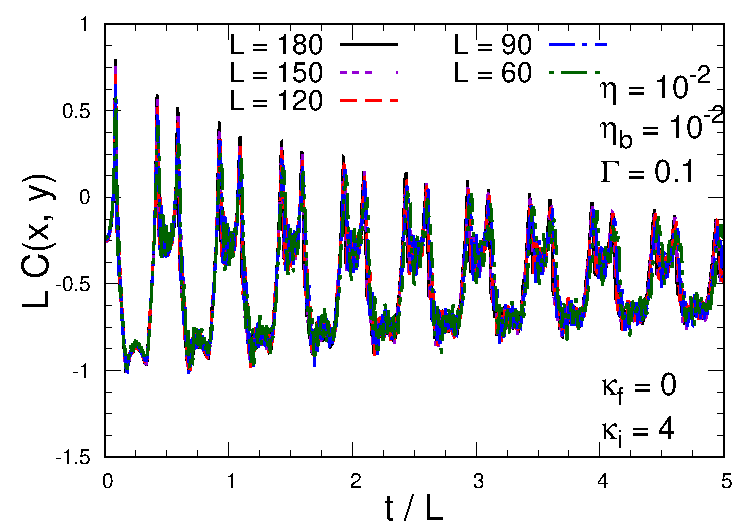
\includegraphics[width=0.95\columnwidth]
    {figs/LCk4q0e001t001S0100.pdf}
  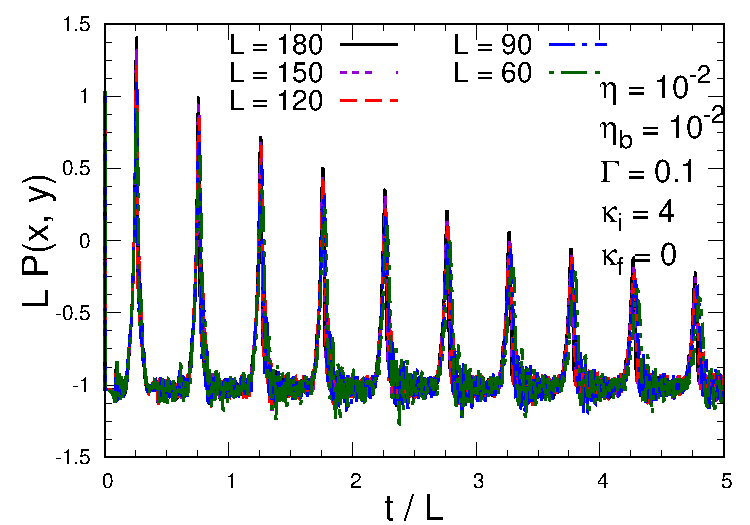
\includegraphics[width=0.95\columnwidth]
    {../data/LPk4q0e001t001S0100.pdf}
  \caption{Scaling behavior of the two-points
    correlations functions $C(x,y,t)$ (top) and $P(x,y,t)$
    (bottom) for $x=L/3$, $y=2L/3$  keeping the scaling
    variables $\kappa_i=-1$, $\kappa=0$, $\Xi =0.01$,
    $\Xi_b=0.01$, $\Gamma=1$ fixed in function of
    $tL^{-z}$, up to system size $L=180$.}
  \label{k4q0e001t001S0100}
\end{figure}

\begin{figure}[!htb]
  \includegraphics[width=0.95\columnwidth]
    {../data/LCk1q0e200t200S1000.pdf}
  \includegraphics[width=0.95\columnwidth]
    {../data/LPk1q0e200t200S1000.pdf}
  \caption{Scaling behavior of the two-points
    correlations functions $C(x,y,t)$ (top) and $P(x,y,t)$
    (bottom) for $x=L/3$, $y=2L/3$  keeping the scaling
    variables $\kappa_i=1$, $\kappa=0$, $\Xi =2$,
    $\Xi_b=2$, $\Gamma=1$ fixed in function of
    $tL^{-z}$, up to system size $L=180$.}
  \label{k1q0e200t200S1000}
\end{figure}

\begin{figure}[!htb]
  \includegraphics[width=0.95\columnwidth]
    {../data/LCk2q0e050t050g0500.pdf}
  \includegraphics[width=0.95\columnwidth]
    {../data/LPk2q0e050t050g0500.pdf}
  \caption{Scaling behavior of the two-points
    correlations functions $C(x,y,t)$ (top) and $P(x,y,t)$
    (bottom) for $x=L/3$, $y=2L/3$  keeping the scaling
    variables $\kappa_i=2$, $\kappa=0$, $\Xi =0.5$,
    $\Xi_b=0.5$, $\gamma=0.5$ fixed in function of
    $tL^{-z}$, up to system size $L=180$.}
  \label{k2q0e050t050g0500}
\end{figure}

\begin{figure}[!htb]
  \includegraphics[width=0.95\columnwidth]
    {../data/Dk1q0e200t200S1000.pdf}
  \includegraphics[width=0.95\columnwidth]
    {../data/Dk2q0e050t050g0500.pdf}
  \caption{Scaling behavior of the particle
   density $D(t)$ minus the value at the critical valueD(0)
    (bottom) for $x=L/3$, $y=2L/3$  keeping the scaling
    variables $\kappa_i=2$, $\kappa=0$, $\Xi =0.5$,
    $\Xi_b=0.5$, $\gamma=0.5$ fixed in function of
    $tL^{-z}$, up to system size $L=180$.}
  \label{k2q0e050t050g0500}
\end{figure}

\end{comment}

\end{document}
